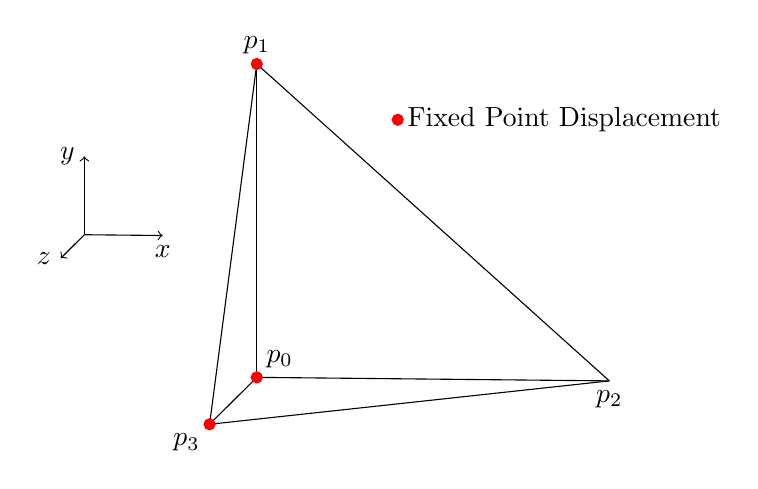
\begin{tikzpicture}
\draw[->] (-0.980017,2.03987) -- (0.0149875,2.0299);
\node[below] at (0.0149875,2.0299) {$x$};
\draw[->] (-0.980017,2.03987) -- (-0.980017,3.03487);
\node[left] at (-0.980017,3.03487) {$y$};
\draw[->] (-0.980017,2.03987) -- (-1.27952,1.74186);
\node[left] at (-1.27952,1.74186) {$z$};
\draw (1.20966,0.228594) -- (1.20966,4.20861);
\draw (1.20966,4.20861) -- (5.68718,0.183744);
\draw (5.68718,0.183744) -- (1.20966,0.228594);
\draw (0.610658,-0.367414) -- (1.20966,0.228594);
\draw (0.610658,-0.367414) -- (1.20966,4.20861);
\draw (0.610658,-0.367414) -- (5.68718,0.183744);
\draw[fill,red] (1.20966,0.228594) circle(0.07);
\node[above right] at (1.20966,0.228594) {$p_0$};
\draw[fill,red] (1.20966,4.20861) circle(0.07);
\node[above] at (1.20966,4.20861) {$p_1$};
\node[below] at (5.68718,0.183744) {$p_2$};
\draw[fill,red] (0.610658,-0.367414) circle(0.07);
\node[below left] at (0.610658,-0.367414) {$p_3$};
\draw[fill,red] (3,3.5) circle(0.07);
\node[right] at (3,3.5) {Fixed Point Displacement};
\end{tikzpicture}